\section{Atomorbitale}
\authors{Johannes Wörsdörfer, Ali Serour}

Atomorbitale sind Einteilchen-Wellenfunktionen. Sie sind Lösungen der Schrödingergleichung für das Wasserstoffatom beziehungsweise für Ionen mit nur einem Elektron. Die Aufenthaltswahrscheinlichkeitsdichte der Elektronen ergibt sich aus dem Betragsquadrat der Funktion. Demnach erwies sich die Vorstellung, dass sich die Elektronen eines Atoms in Schalen bewegen, als unvollständig. Darauf wird im Kapitel Schrödingergleichung  näher eingegangen.

Atomorbitale werden mithilfe von vier Quantenzahlen klassifiziert. Die Hauptquantenzahl $n$ definiert das Energieniveau des Elektrons. Die Nebenquantenzahl $l$ bestimmt die Geometrie der Orbitale. Sie kann die Werte $l = 0, 1, ..., n-1$ annehmen. Die magnetische Quantenzahl $m$ beschreibt den Drehimpuls eines Elektrons und somit die Ausrichtung des Orbitals im Raum. Es gibt die magnetischen Quantenzahlen $m = -l,...,l$. Die vierte Zahl ist die Spinquantenzahl $s$. Diese kann die Werte $s = -\frac{1}{2}, \frac{1}{2}$ annehmen \cite{Riedel07}. 

Um größere Atome beschreiben zu können, bedienen wir uns einer Näherung: Wir konstruieren die Vielteilchenwellenfunktion mithilfe von Einteilchenwellenfunktionen, die mit Elektronen besetzt werden. Dabei müssen drei Regeln beachtet werden: Das Aufbauprinzip besagt, dass zuerst alle energieärmeren Niveaus besetzt werden, bevor das darüber liegende Orbital besetzt wird. Die Hundsche Regel schreibt vor, dass bei einer Entartung eines Orbitals zuerst alle Orbitale mit gleicher Nebenquantenzahl $l$ mit dem gleichen Spin besetzt werden. Das Pauli-Prinzip gibt an, dass ein Orbital nur mit zwei Elektronen mit entgegengesetztem Spin besetzt werden kann, da es nicht zwei Elektronen mit exakt den selben Quantenzahlen innerhalb eines Atoms geben darf.

Im Folgenden wird dieses Modell anhand des Kohlenstoffatoms mithilfe eines Energieniveaudiagramms illustriert (siehe Abb. \ref{fig:Energieniveaudiagramm}). Kohlenstoff hat die Ordnungszahl 6. Es besitzt somit 6 Elektronen. Die Orbitale werden von unten nach oben mit Elektronen aufgefüllt, da Elektronen die energetisch günstigste Anordnung anstreben.  Die Elektronenkonfiguration für Kohlenstoff lautet $1s^{2} 2s^{2} 2p^{2}$. Die vorderen Zahlen geben die Hauptquantenzahl an. Der Buchstabe bezeichnet die Nebenquantenzahl der Orbitale mit $s$ für $l = 0$ und $p$ für $l=1$ und der Exponent definiert die Anzahl der Elektronen im jeweiligen Orbital.

\begin{dsafigure}
 \centering
 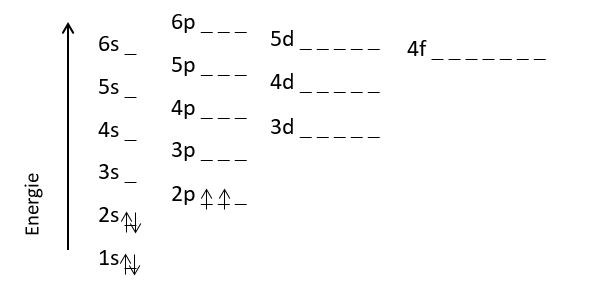
\includegraphics[width=\columnwidth]{Energieniveaudiagramm.png}
 \caption{Die Besetzung der Orbitale nach dem Aufbauprinzip, der Hunschen Regel und dem Pauli-Prinzip ist anhand des Kohlenstoffatoms mithilfe eines Energieniveaudiagramms illustriert.}
 \label{fig:Energieniveaudiagramm}
\end{dsafigure}

Zum besseren Verständnis betrachten wir nun die räumliche Gestalt der Orbitale.
Das s-Orbital hat die Form einer Kugel (siehe Abb. \ref{fig:s}).
Die Nebenquantenzahl beträgt $0$. Außerdem hat es keine Knotenebene. Das
p-Orbital hat die Nebenquantenzahl 1. Es gibt genau drei Magnetquantenzahlen
$m = -1, 0, 1$. Das Orbital mit der magnetischen Quantenzahl $0$ hat die Form
einer Hantel entlang der $z$-Achse. Es wir auch als $p_{z}$ bezeichnet
(siehe Abb. \ref{fig:px_py_pz}). Aus den Zuständen $m = -1$ und $1$ werden
die Linearkombinationen $p_{x} = \frac{1}{\sqrt{2}} (p_{+1} - p_{-1})$
und $p_{y} = \frac{i}{\sqrt{2}}(p_{+1}+p_{-1})$
gebildet. Gleiches lässt sich auch auf
d-Orbitale übertragen (siehe Abb. \ref{fig:dz2} -- \ref{fig:dyz}).

\begin{dsafigure}
 \centering
 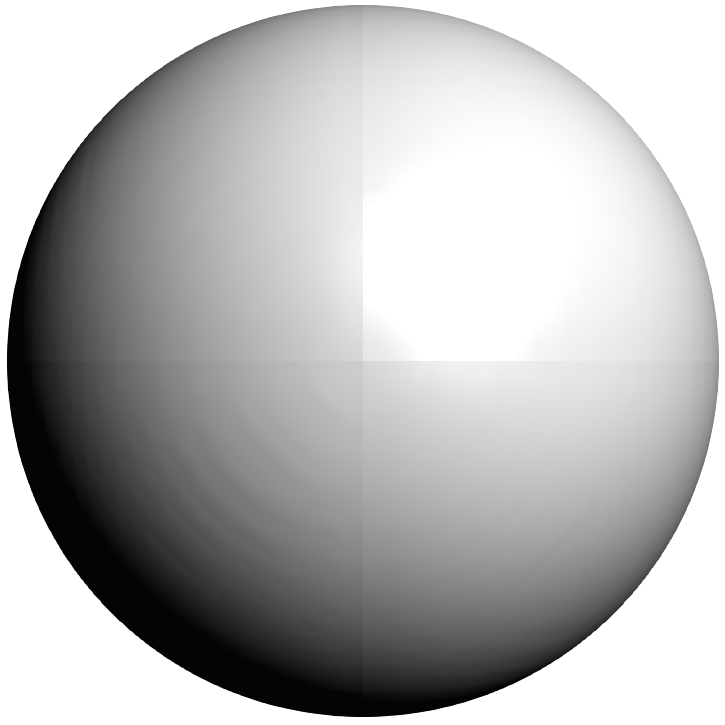
\includegraphics[width=\columnwidth]{s.png}
 \caption{Darstellung eines s-Orbitals \cite{ADF2017authors}.}
 \label{fig:s}
\end{dsafigure}

\begin{dsafigure}
 \centering
 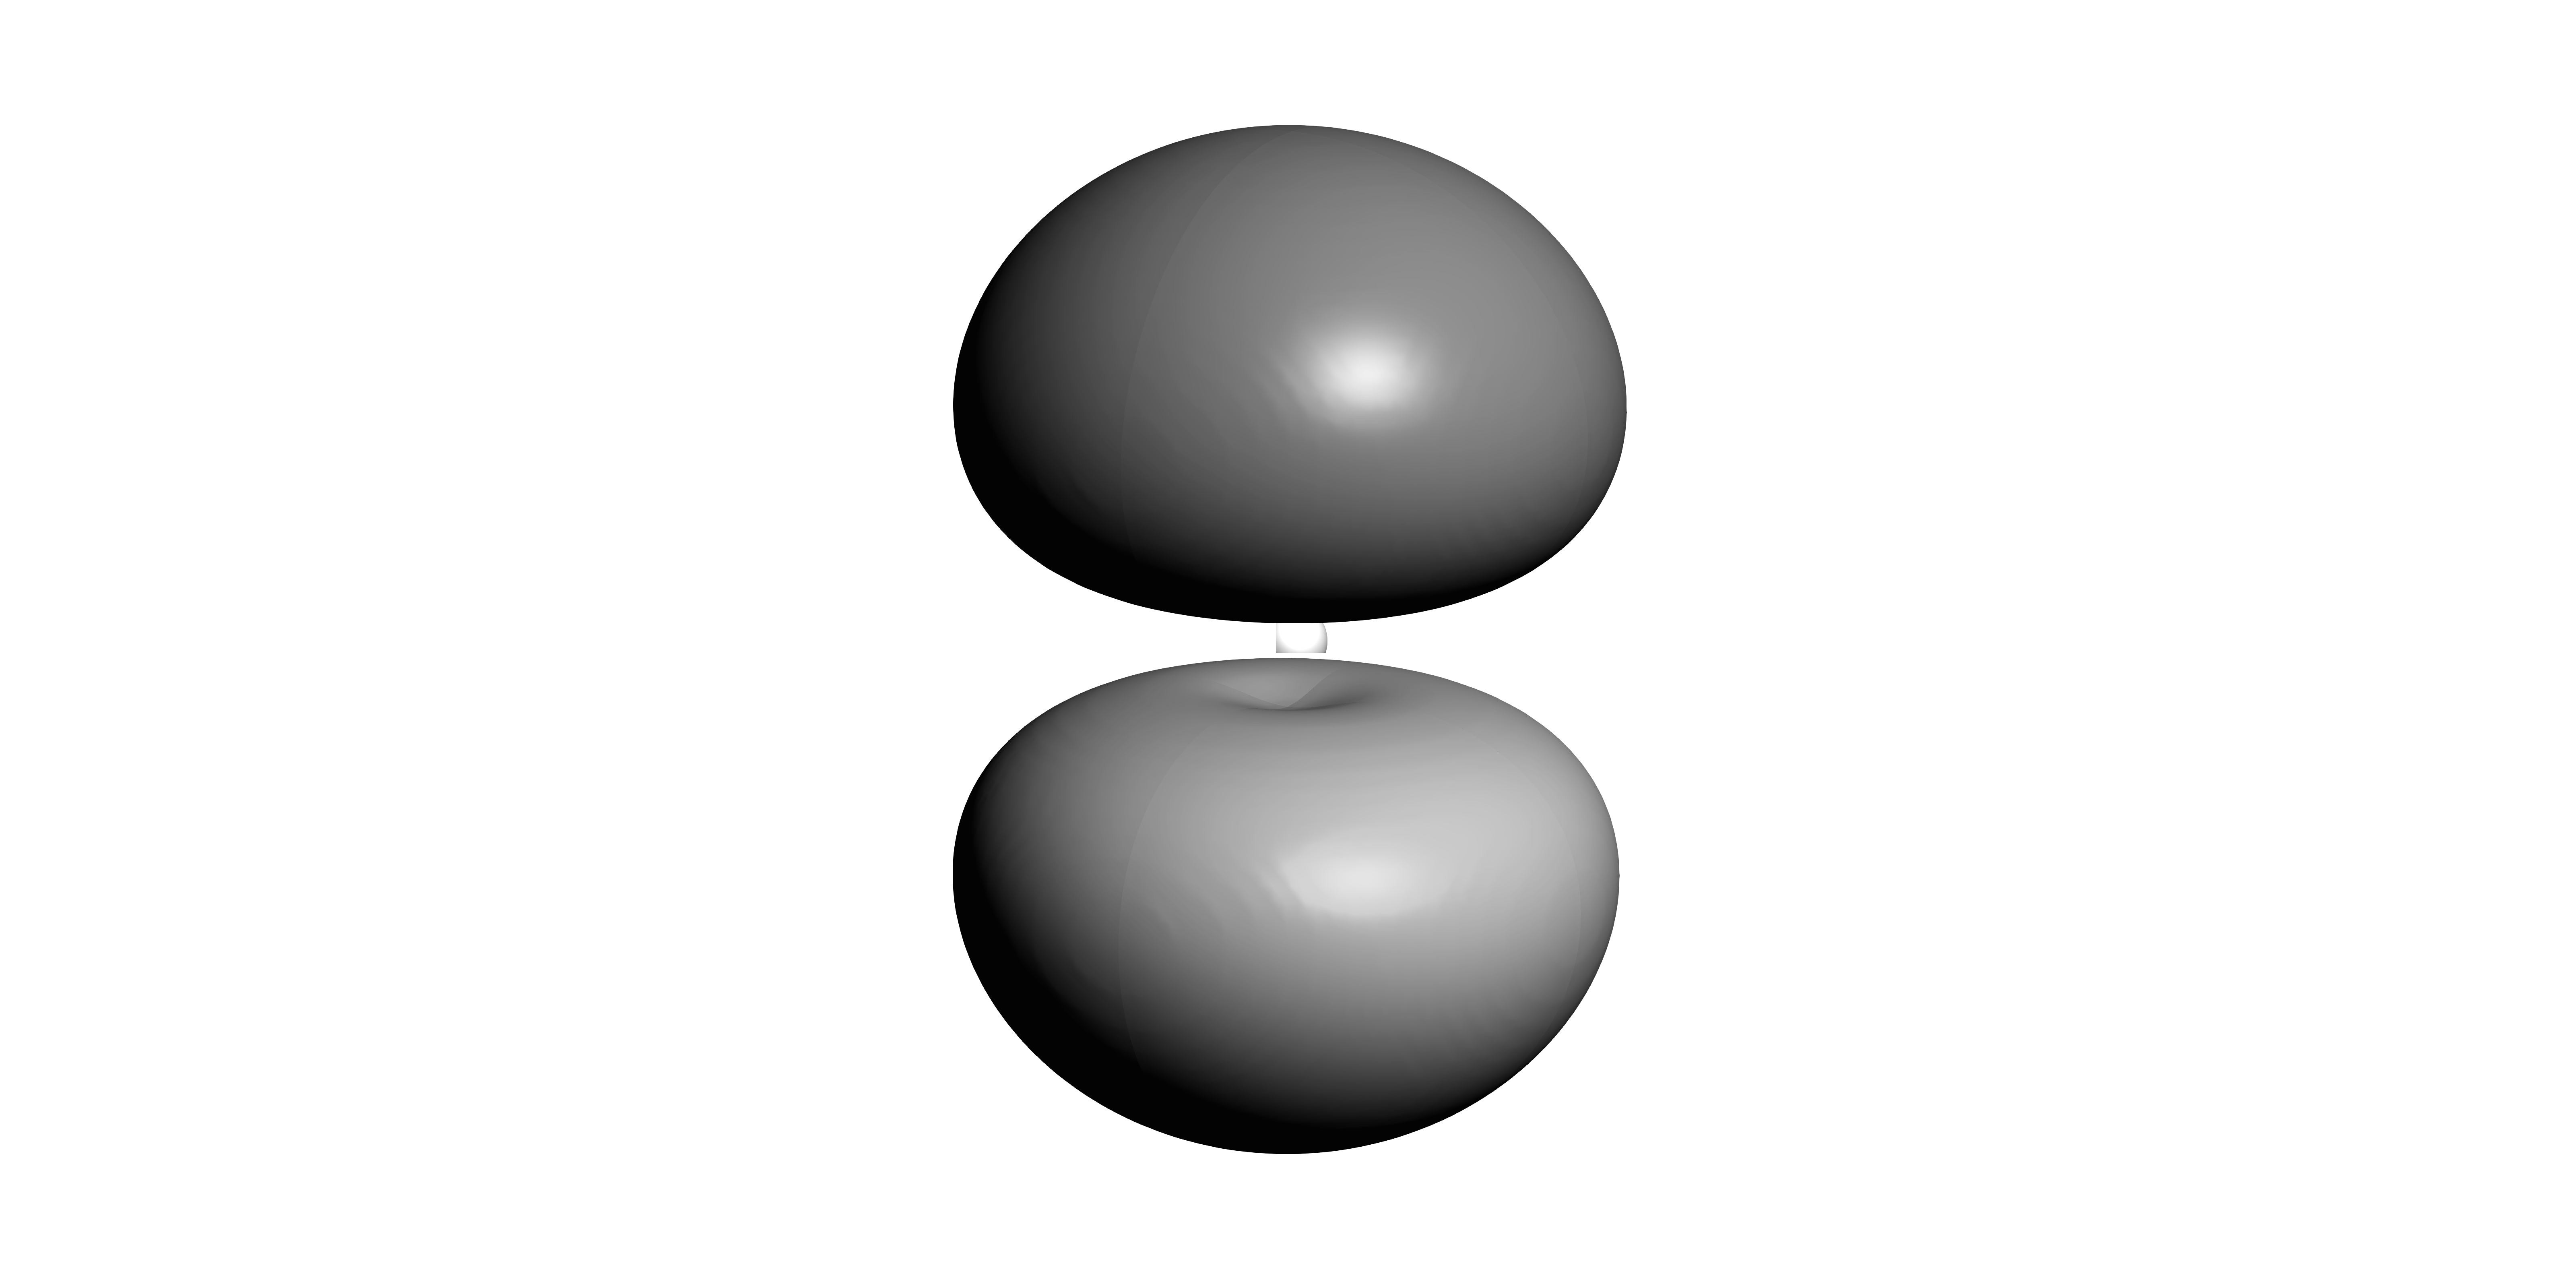
\includegraphics[width=0.25\columnwidth]{pz.png}
 \raisebox{0.5cm}{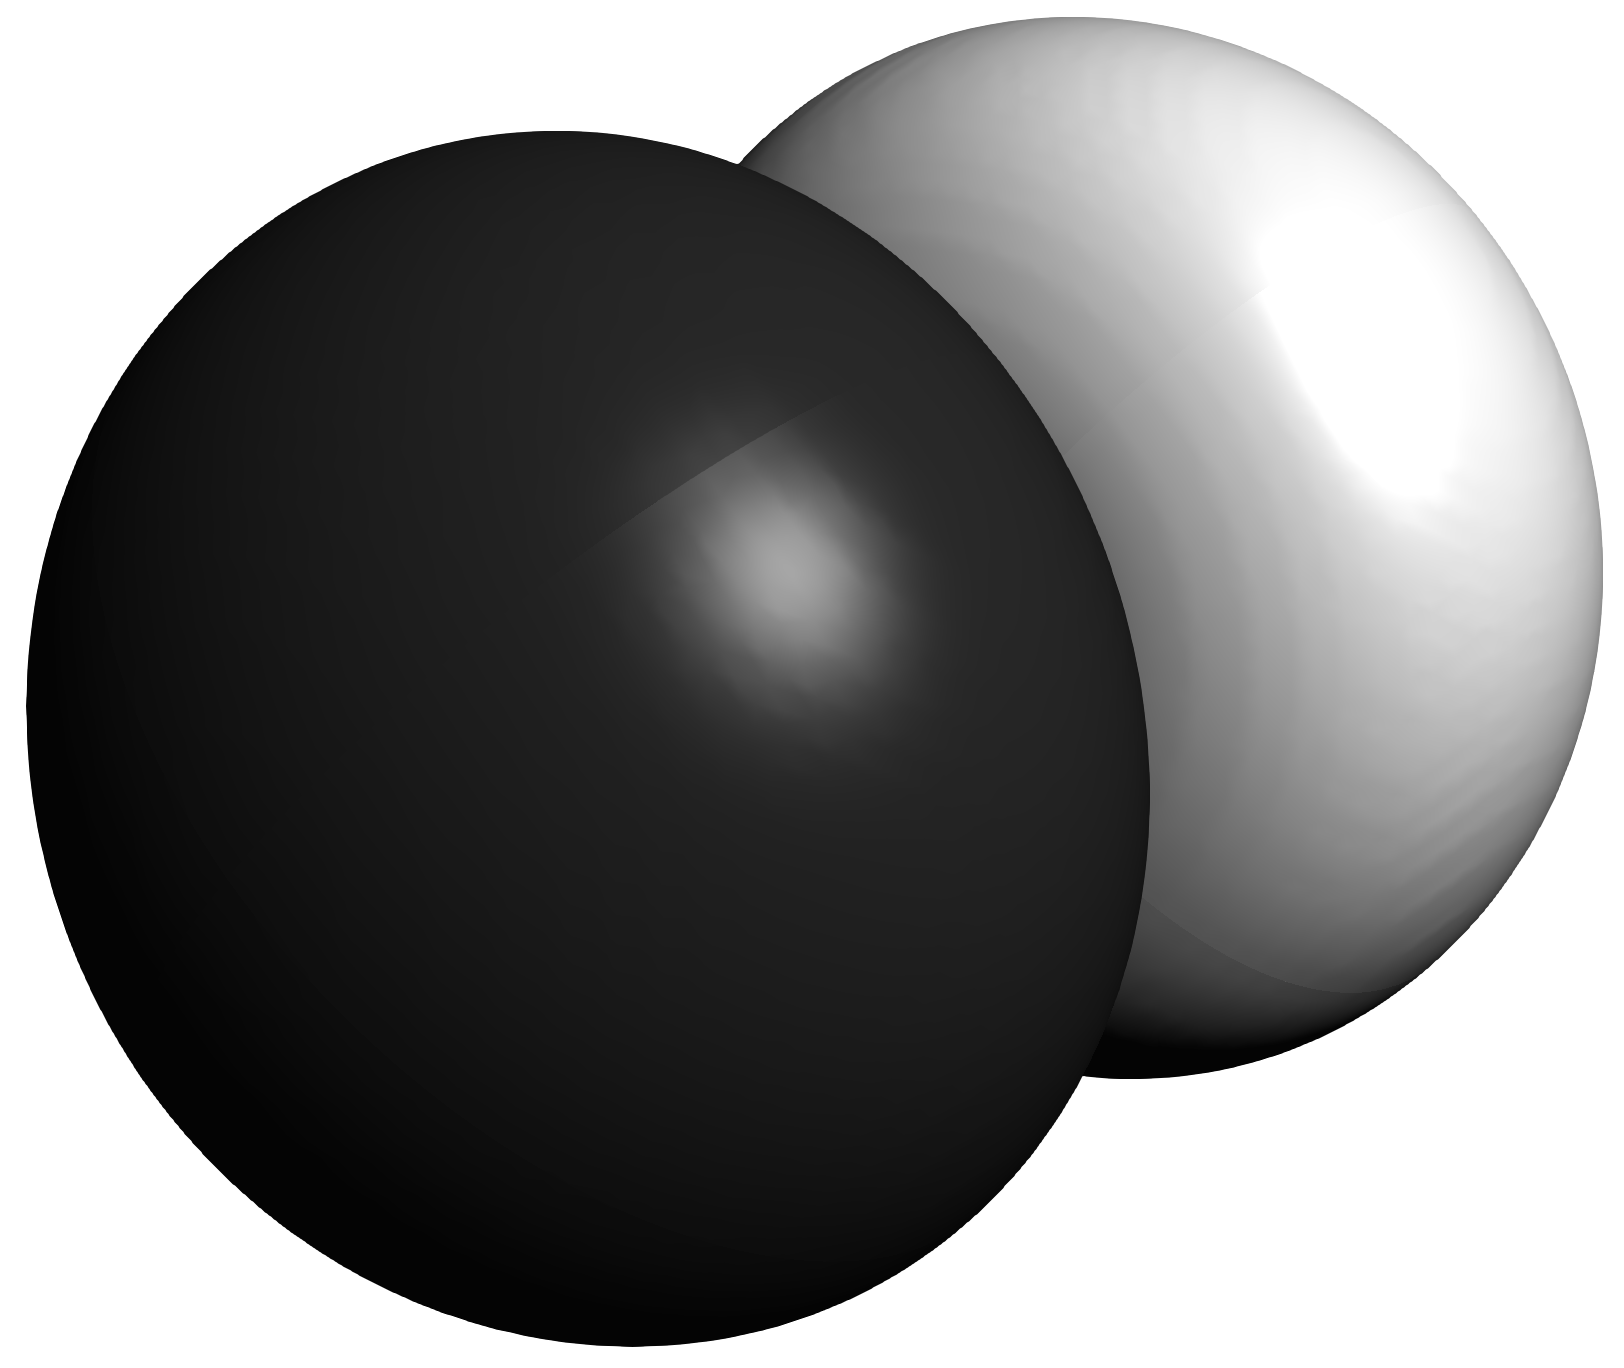
\includegraphics[width=0.3\columnwidth]{px.png}}
 \raisebox{0.5cm}{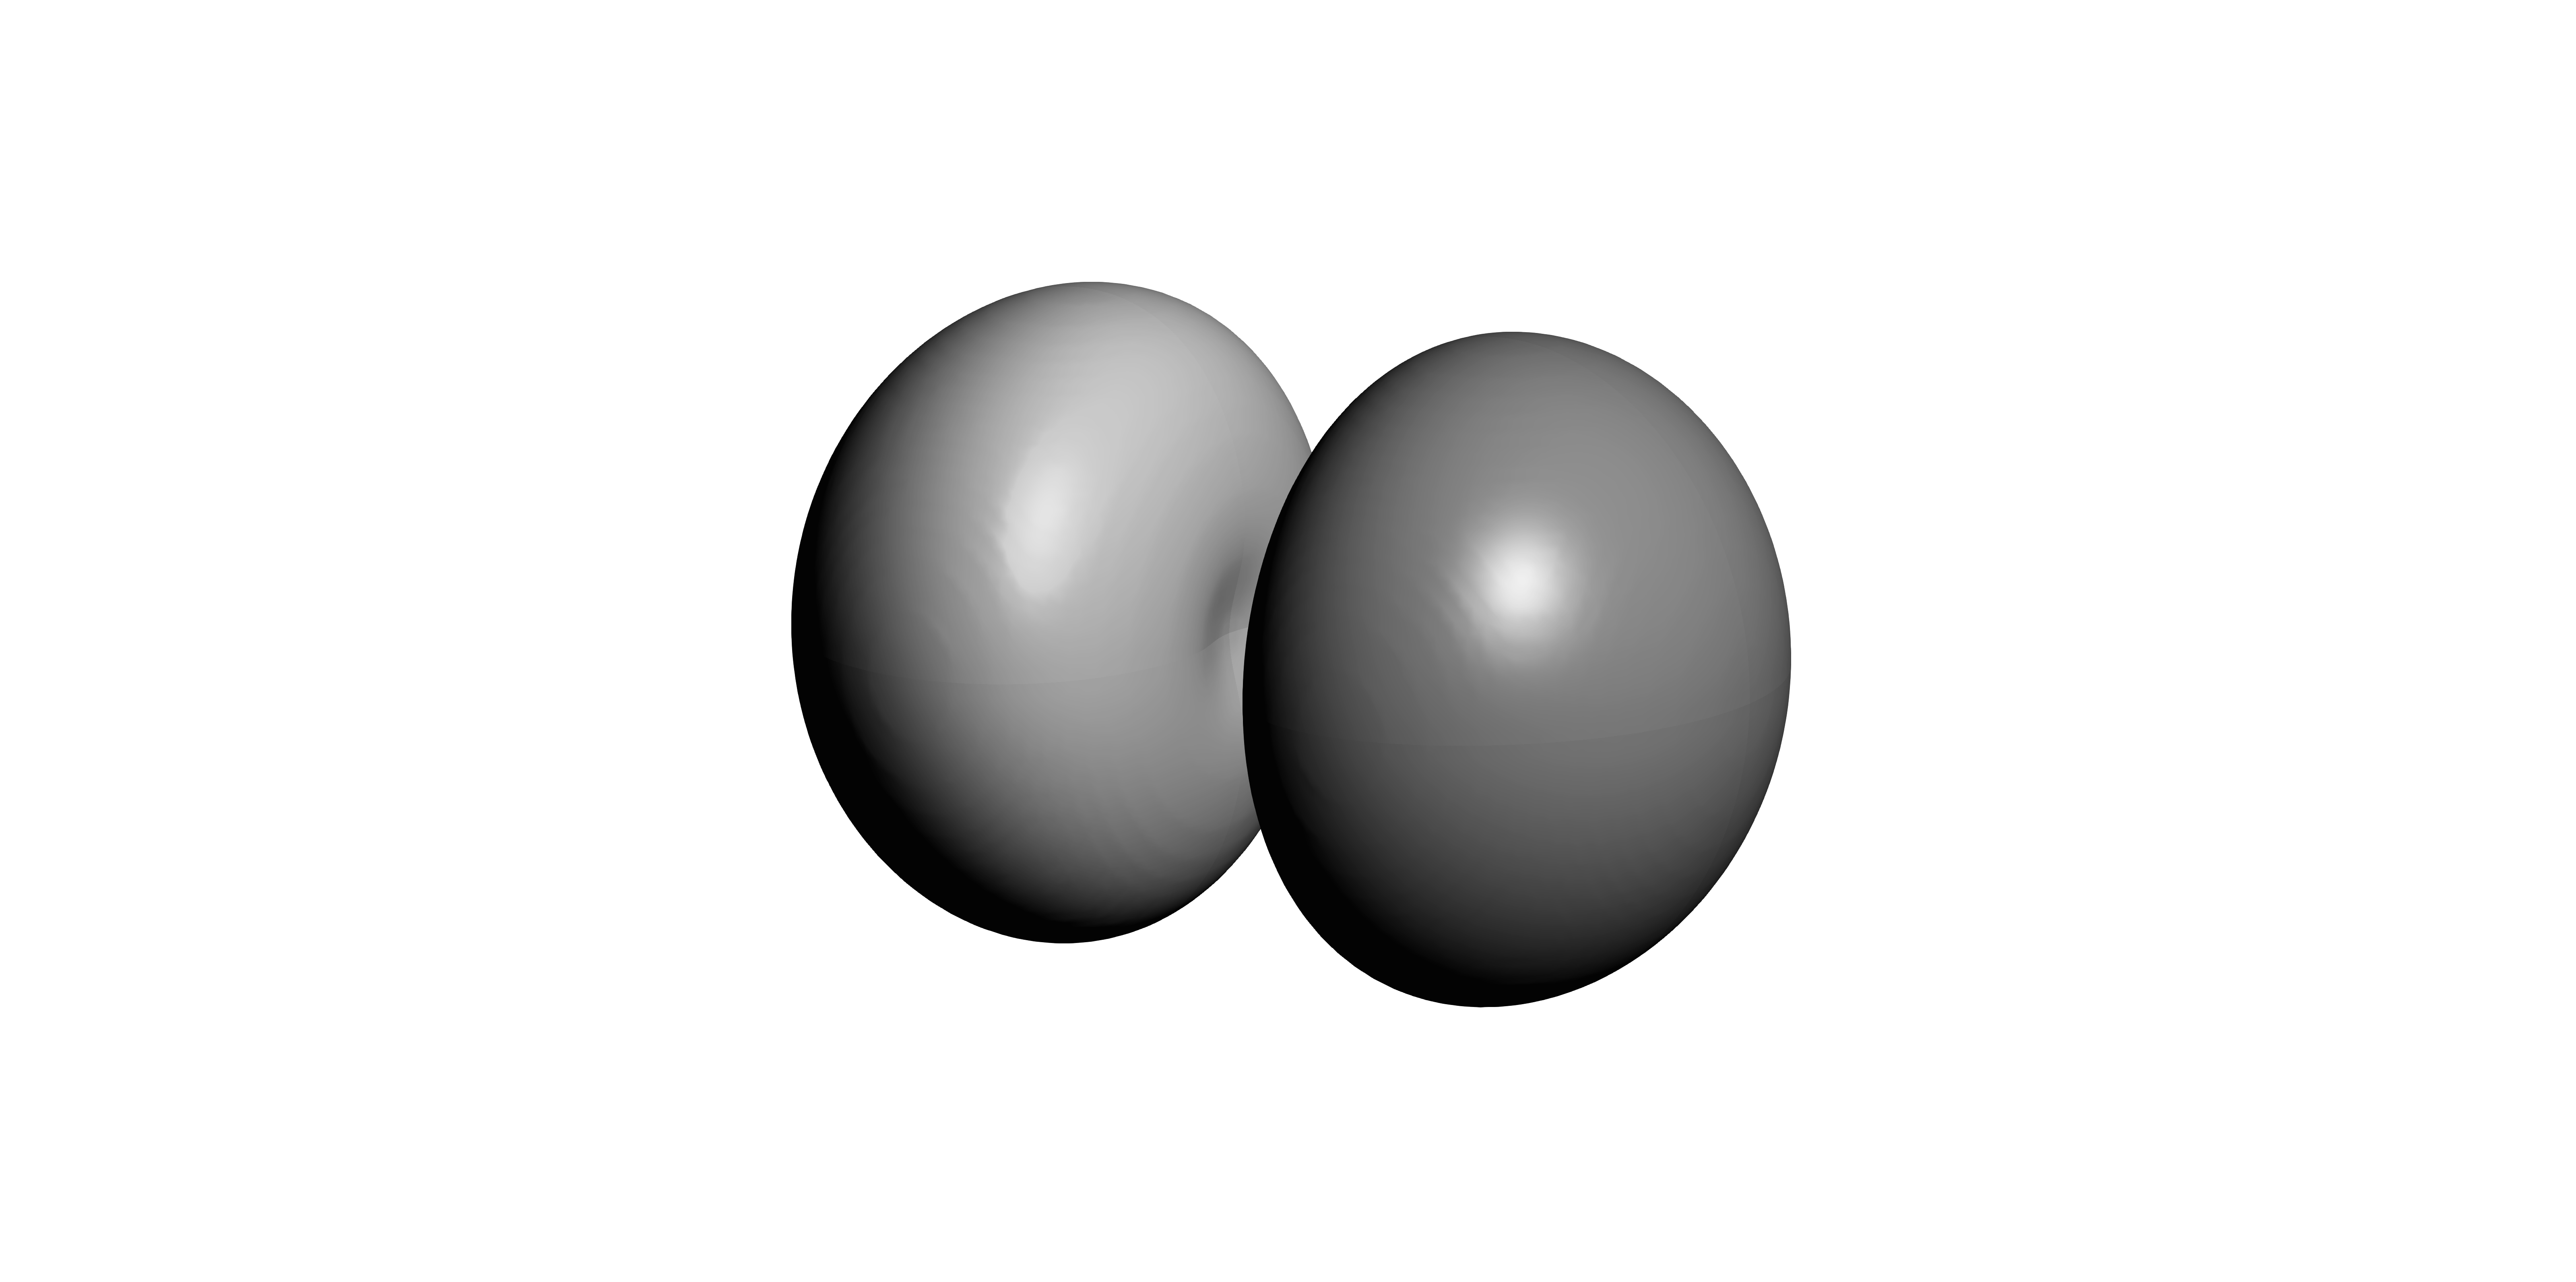
\includegraphics[width=0.31\columnwidth]{py.png}}
 \caption{Darstellung eines p$_{z}$, p$_{x}$ und p$_{y}$-Orbitals \cite{ADF2017authors}.}
 \label{fig:px_py_pz}
\end{dsafigure}

\begin{dsafigure}
 \centering
 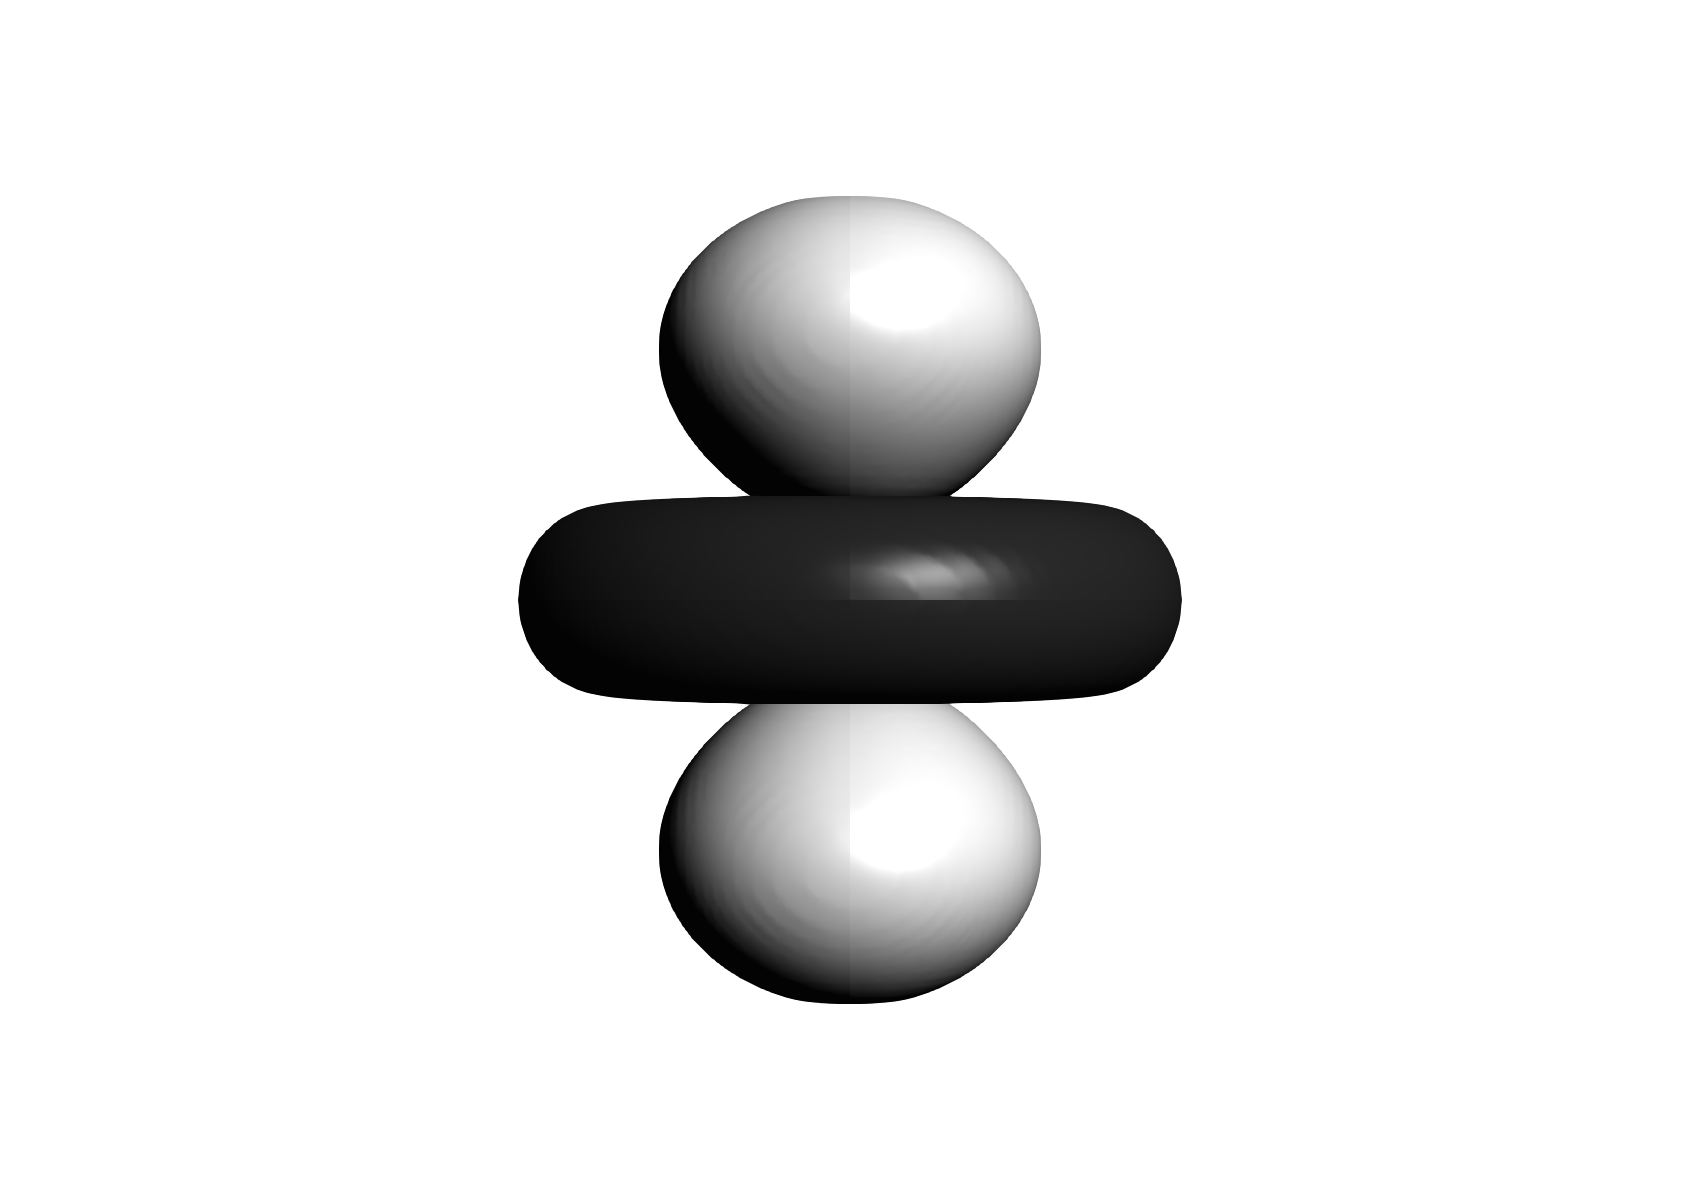
\includegraphics[width=\columnwidth]{dz2.png}
 \caption{Darstellung eines d$_{z^{2}}$-Orbitals \cite{ADF2017authors}.}
 \label{fig:dz2}
\end{dsafigure}

\begin{dsafigure}
 \centering
 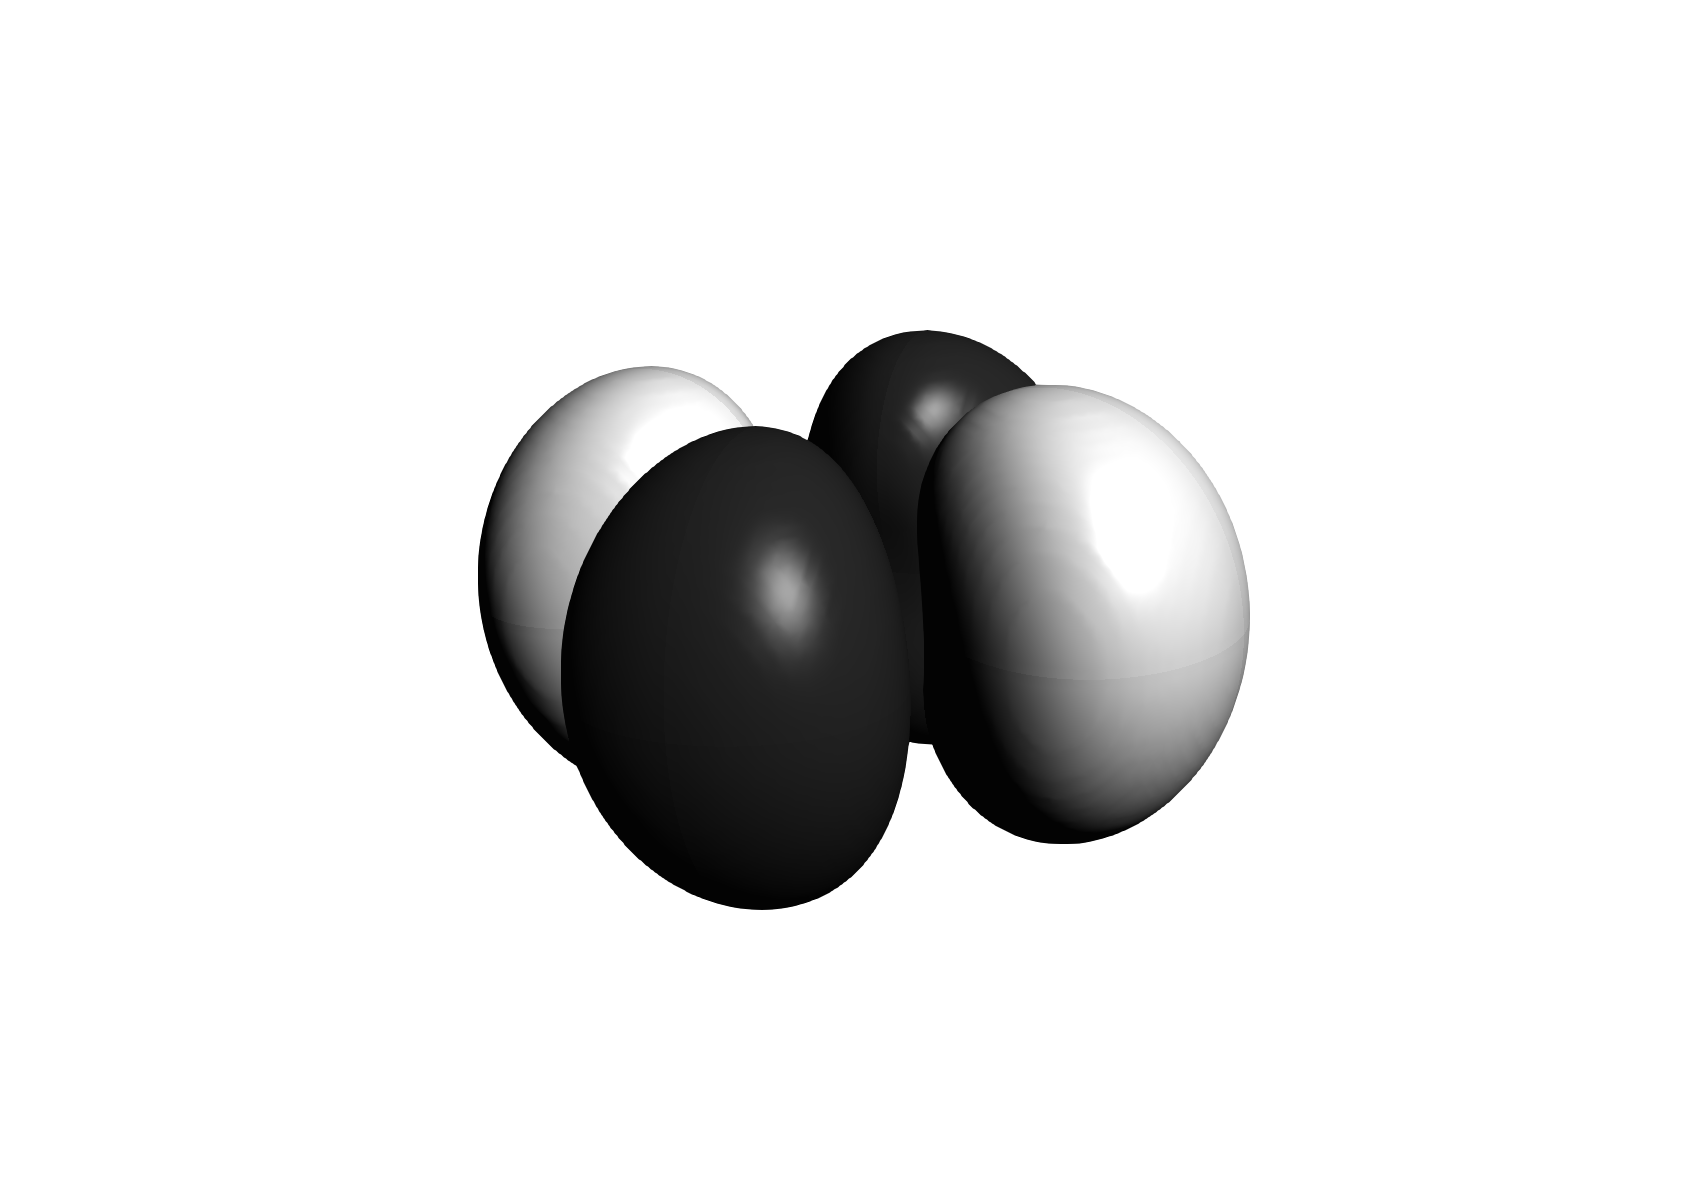
\includegraphics[width=\columnwidth]{dx2-y2.png}
 \caption{Darstellung eines d$_{x^{2}-y^{2}}$-Orbitals \cite{ADF2017authors}.}
 \label{fig:dx2-y2}
\end{dsafigure}

\begin{dsafigure}
 \centering
 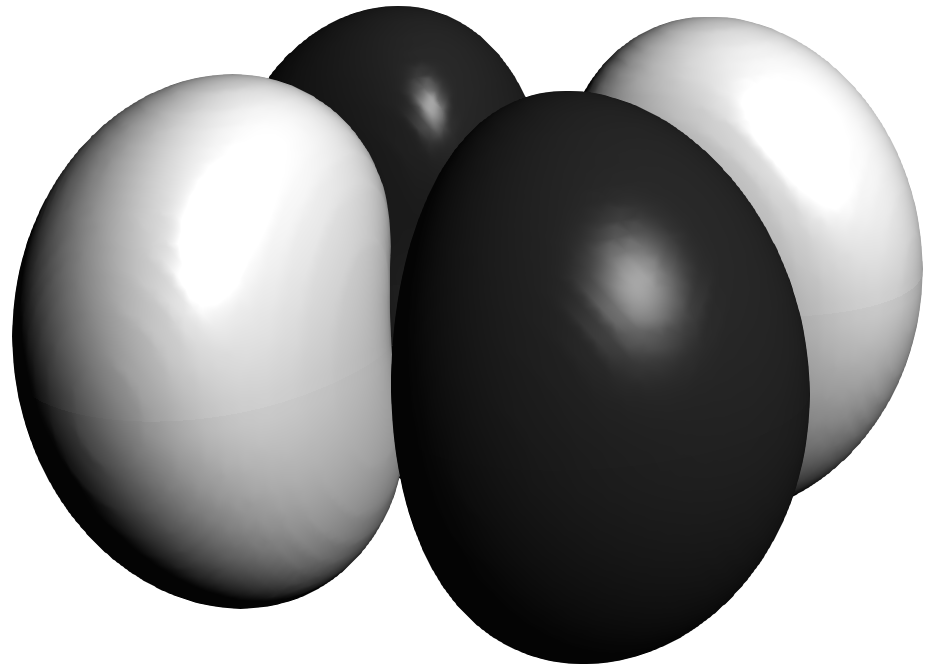
\includegraphics[width=\columnwidth]{dxy.png}
 \caption{Darstellung eines d$_{xy}$-Orbitals \cite{ADF2017authors}.}
 \label{fig:dxy}
\end{dsafigure}

\begin{dsafigure}
 \centering
 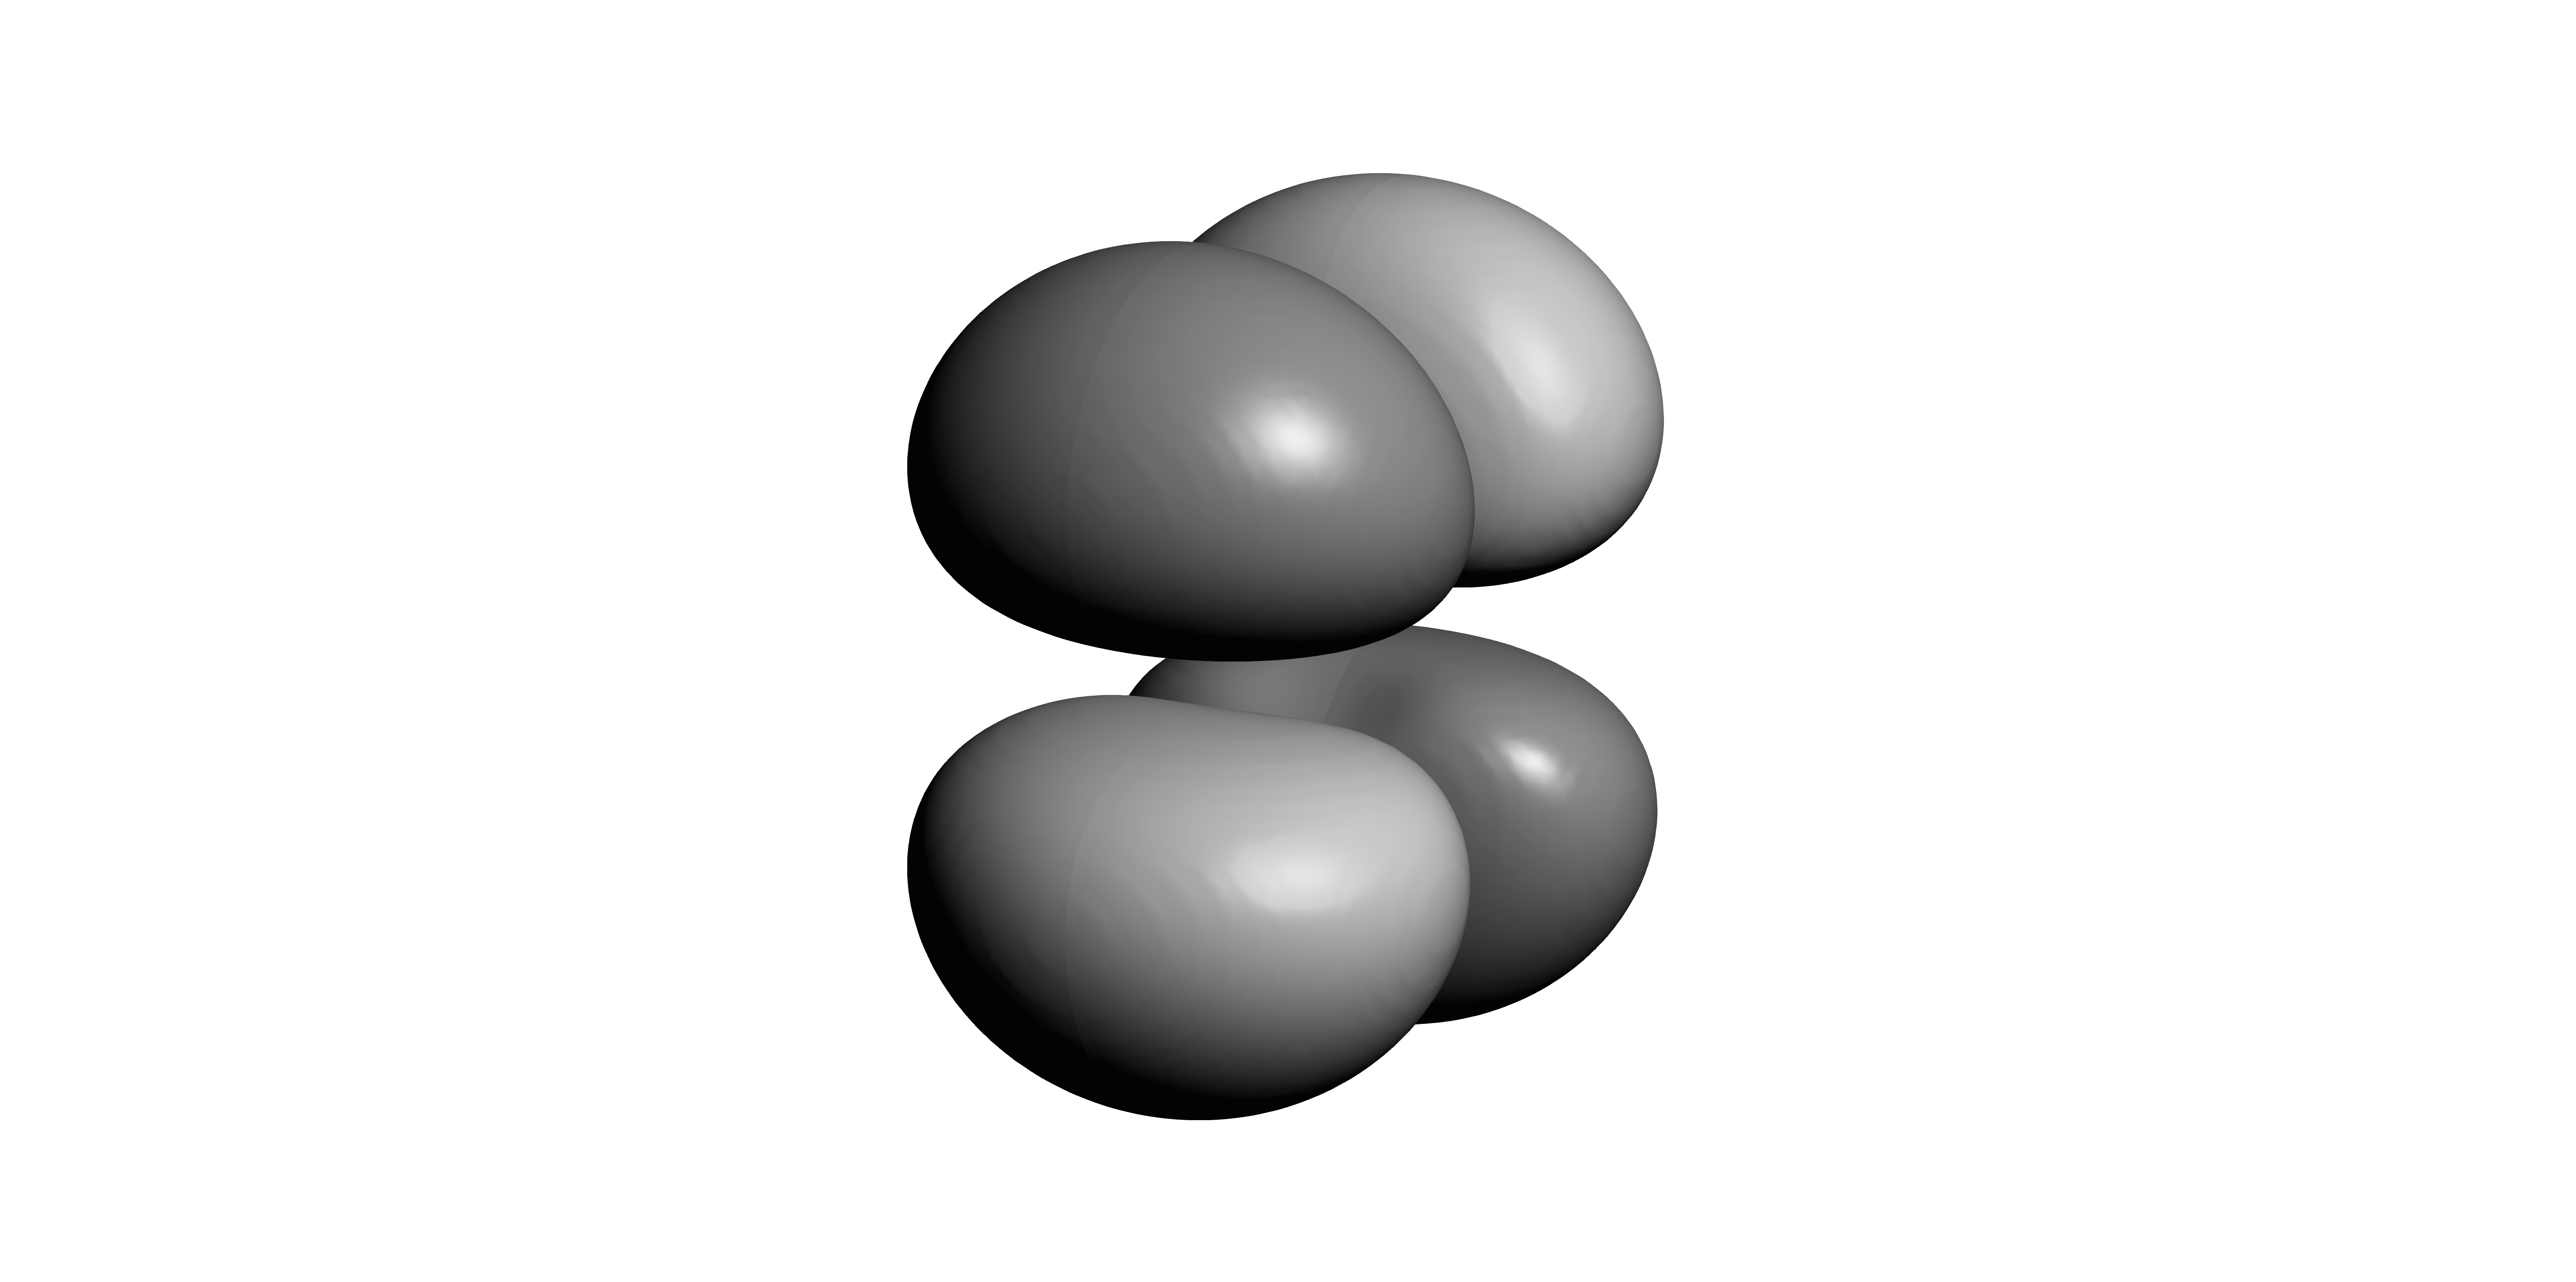
\includegraphics[width=\columnwidth]{dxz.png}
 \caption{Darstellung eines d$_{xz}$-Orbitals \cite{ADF2017authors}.}
 \label{fig:dxz}
\end{dsafigure}

\begin{dsafigure}
 \centering
 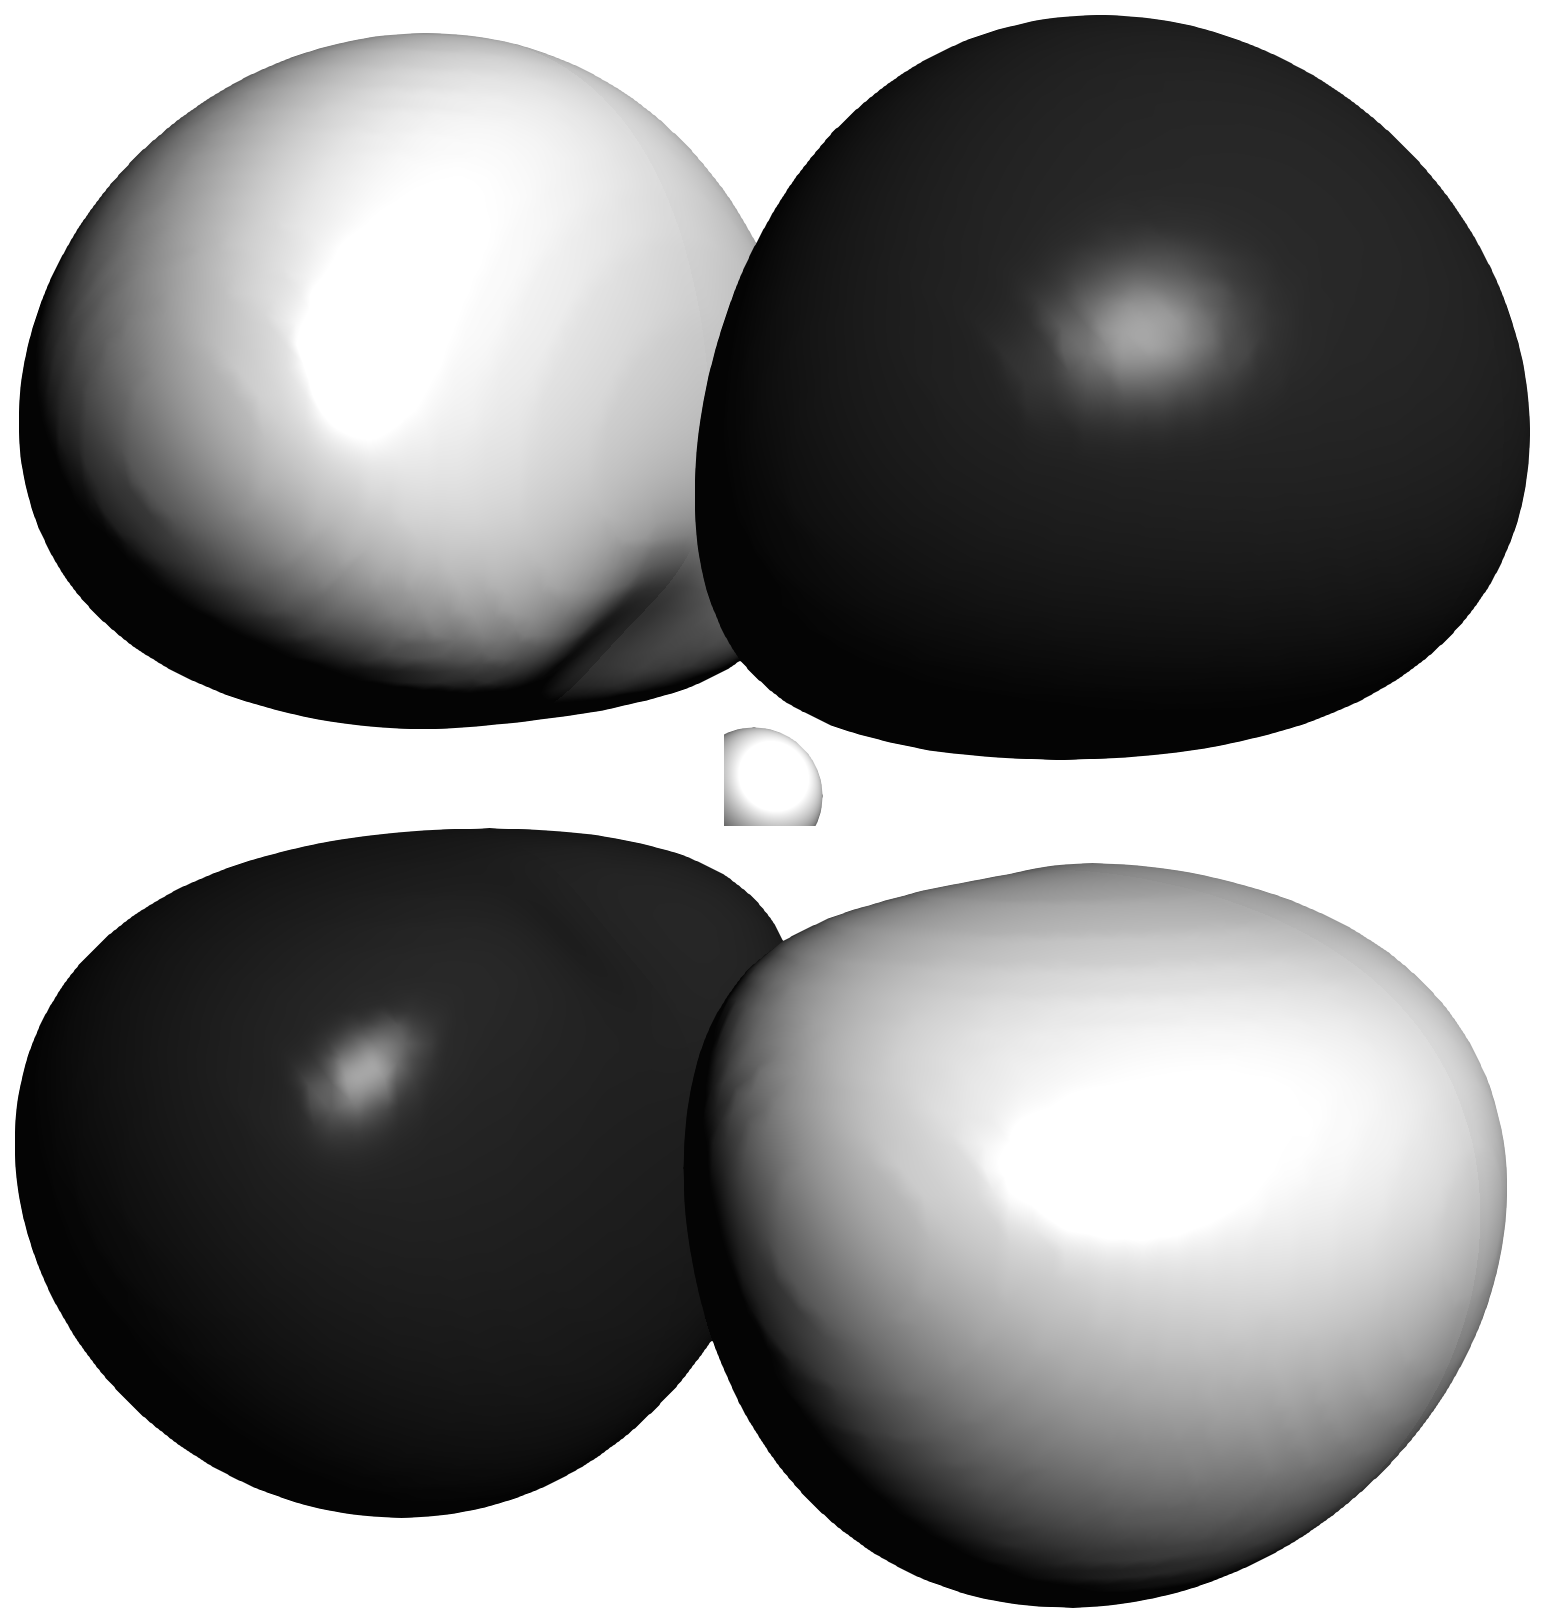
\includegraphics[width=\columnwidth]{dyz.png}
 \caption{Darstellung eines d$_{yz}$-Orbitals \cite{ADF2017authors}.}
 \label{fig:dyz}
\end{dsafigure}

